\providecommand\ExamFontPath{../../../字体/}
\documentclass[fontset=exam]{exam-zh}
\usepackage{longtable,booktabs,array,calc,multirow,fvextra}
\usepackage[normalem]{ulem}
\providecommand{\hl}[1]{#1}
\providecommand{\ul}[1]{\uline{#1}}
\DefineVerbatimEnvironment{verbatim}{Verbatim}{breaklines=true,fontsize=\small}
\providecommand{\tightlist}{\setlength{\itemsep}{0pt}\setlength{\parskip}{0pt}}
\newcommand{\pandocbounded}[1]{#1}
\setlength{\emergencystretch}{3em}
\setlength{\tabcolsep}{2pt}
\examsetup{page/size=a4paper}
\title{厦门大学 2012—2013 年 期末考试}
\subject[4em]{热学}
\begin{document}
\maketitle
\fancyfoot[C]{第 \thepage 页（共 \pageref*{LastPage} 页）}
1.（15 分）

体积为\(V = 2\,\text{L}\)的容器中储存有 2mol 的氧气，今测得分子的平均速率\(\overline{v} = 500\text{m}\text{/}\text{s}\)。求：

（1）系统的温度和压强；

（2）系统的内能。

2.（15 分）

体积为\emph{V}的容器中含有\emph{N}个质量均为\emph{m}的单原子分子，其分子速率分布函数为\(f(v)\)，试写出计算下列各物理量的表达式：

（1）速率大于\(v_{0}\)的分子数；

（2）速率大于\(v_{0}\)的分子的平均速率；

（3）系统的内能；

（4）系统的压强。

3.（15 分）

1mol 理想气体分别经以下两个准静态过程从 300K 加热至 350K：

（1）体积保持不变

（2）压强保持不变

设气体的定容摩尔热容\(C_{V,m} = \frac{3}{2}R\)，问这两个过程中各吸收多少热量？增加多少内能？对外做多少功？

4、（15 分）\par\medskip{\centering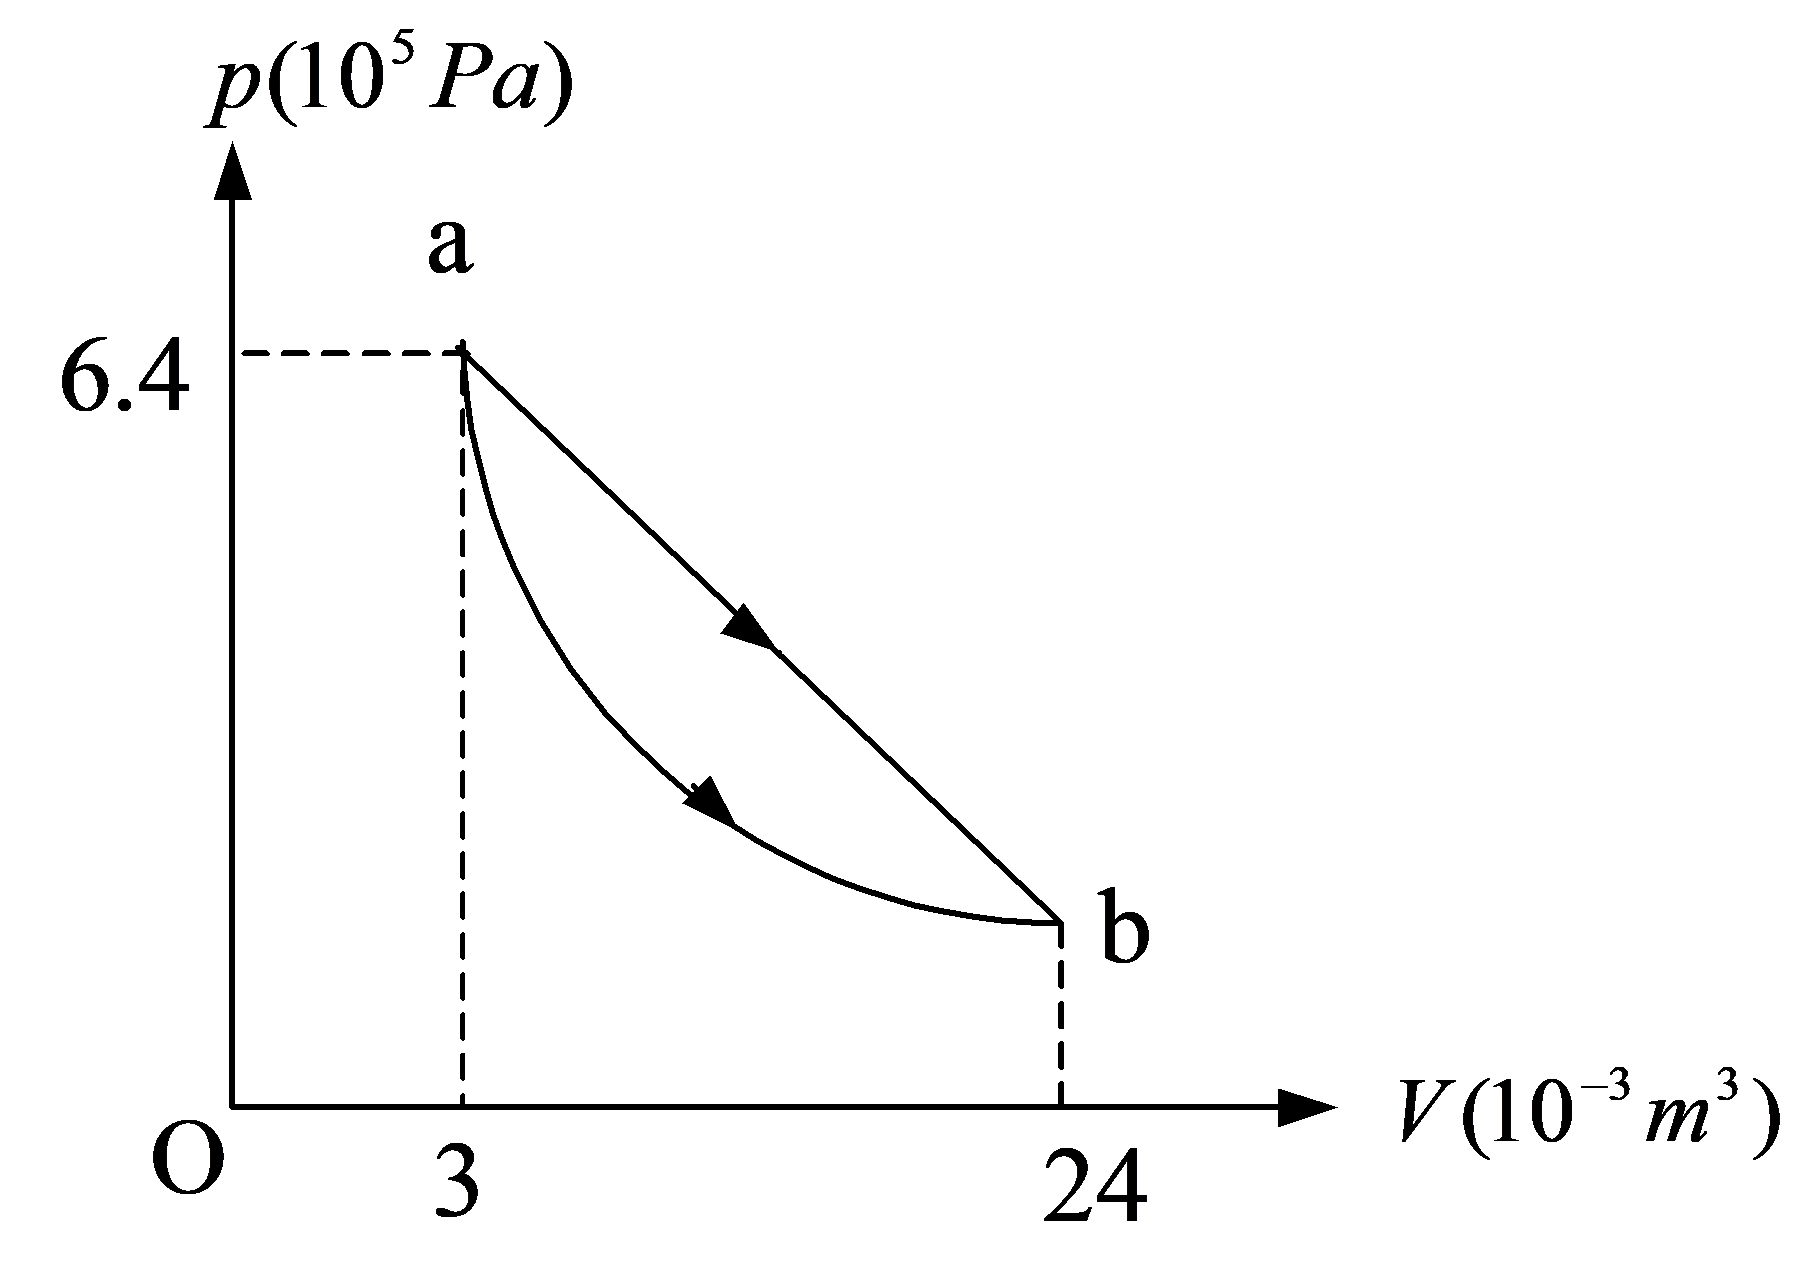
\includegraphics[width=5cm,height=4cm,keepaspectratio]{figures/image20.png}\par}\medskip

如图，某理想气体经一准静态绝热过程从状态 a 过渡到状态 b。设气体的定容摩尔热容\(C_{V,m} = \frac{3}{2}R\)，求系统对外所做的功。如系统经直线过程从 a 过渡到 b，则系统对外做功为多少？与外界之间交换的热量为多少？

5.（15 分）

1mol 理想气体经一准静态过程：\(V = \alpha\,\sqrt{T}\)（\(\alpha\)为常量）。已知该气体的定容摩尔热容量为\(C_{V,m} = \frac{5}{2}R\)（\emph{R}为气体普适为常量），求：

（1）系统温度从\(T_{1}\)变到\(T_{2}\)时气体所做的功\emph{A}；

（2）该过程的摩尔热容\emph{C}。

6．（15 分）\par\medskip{\centering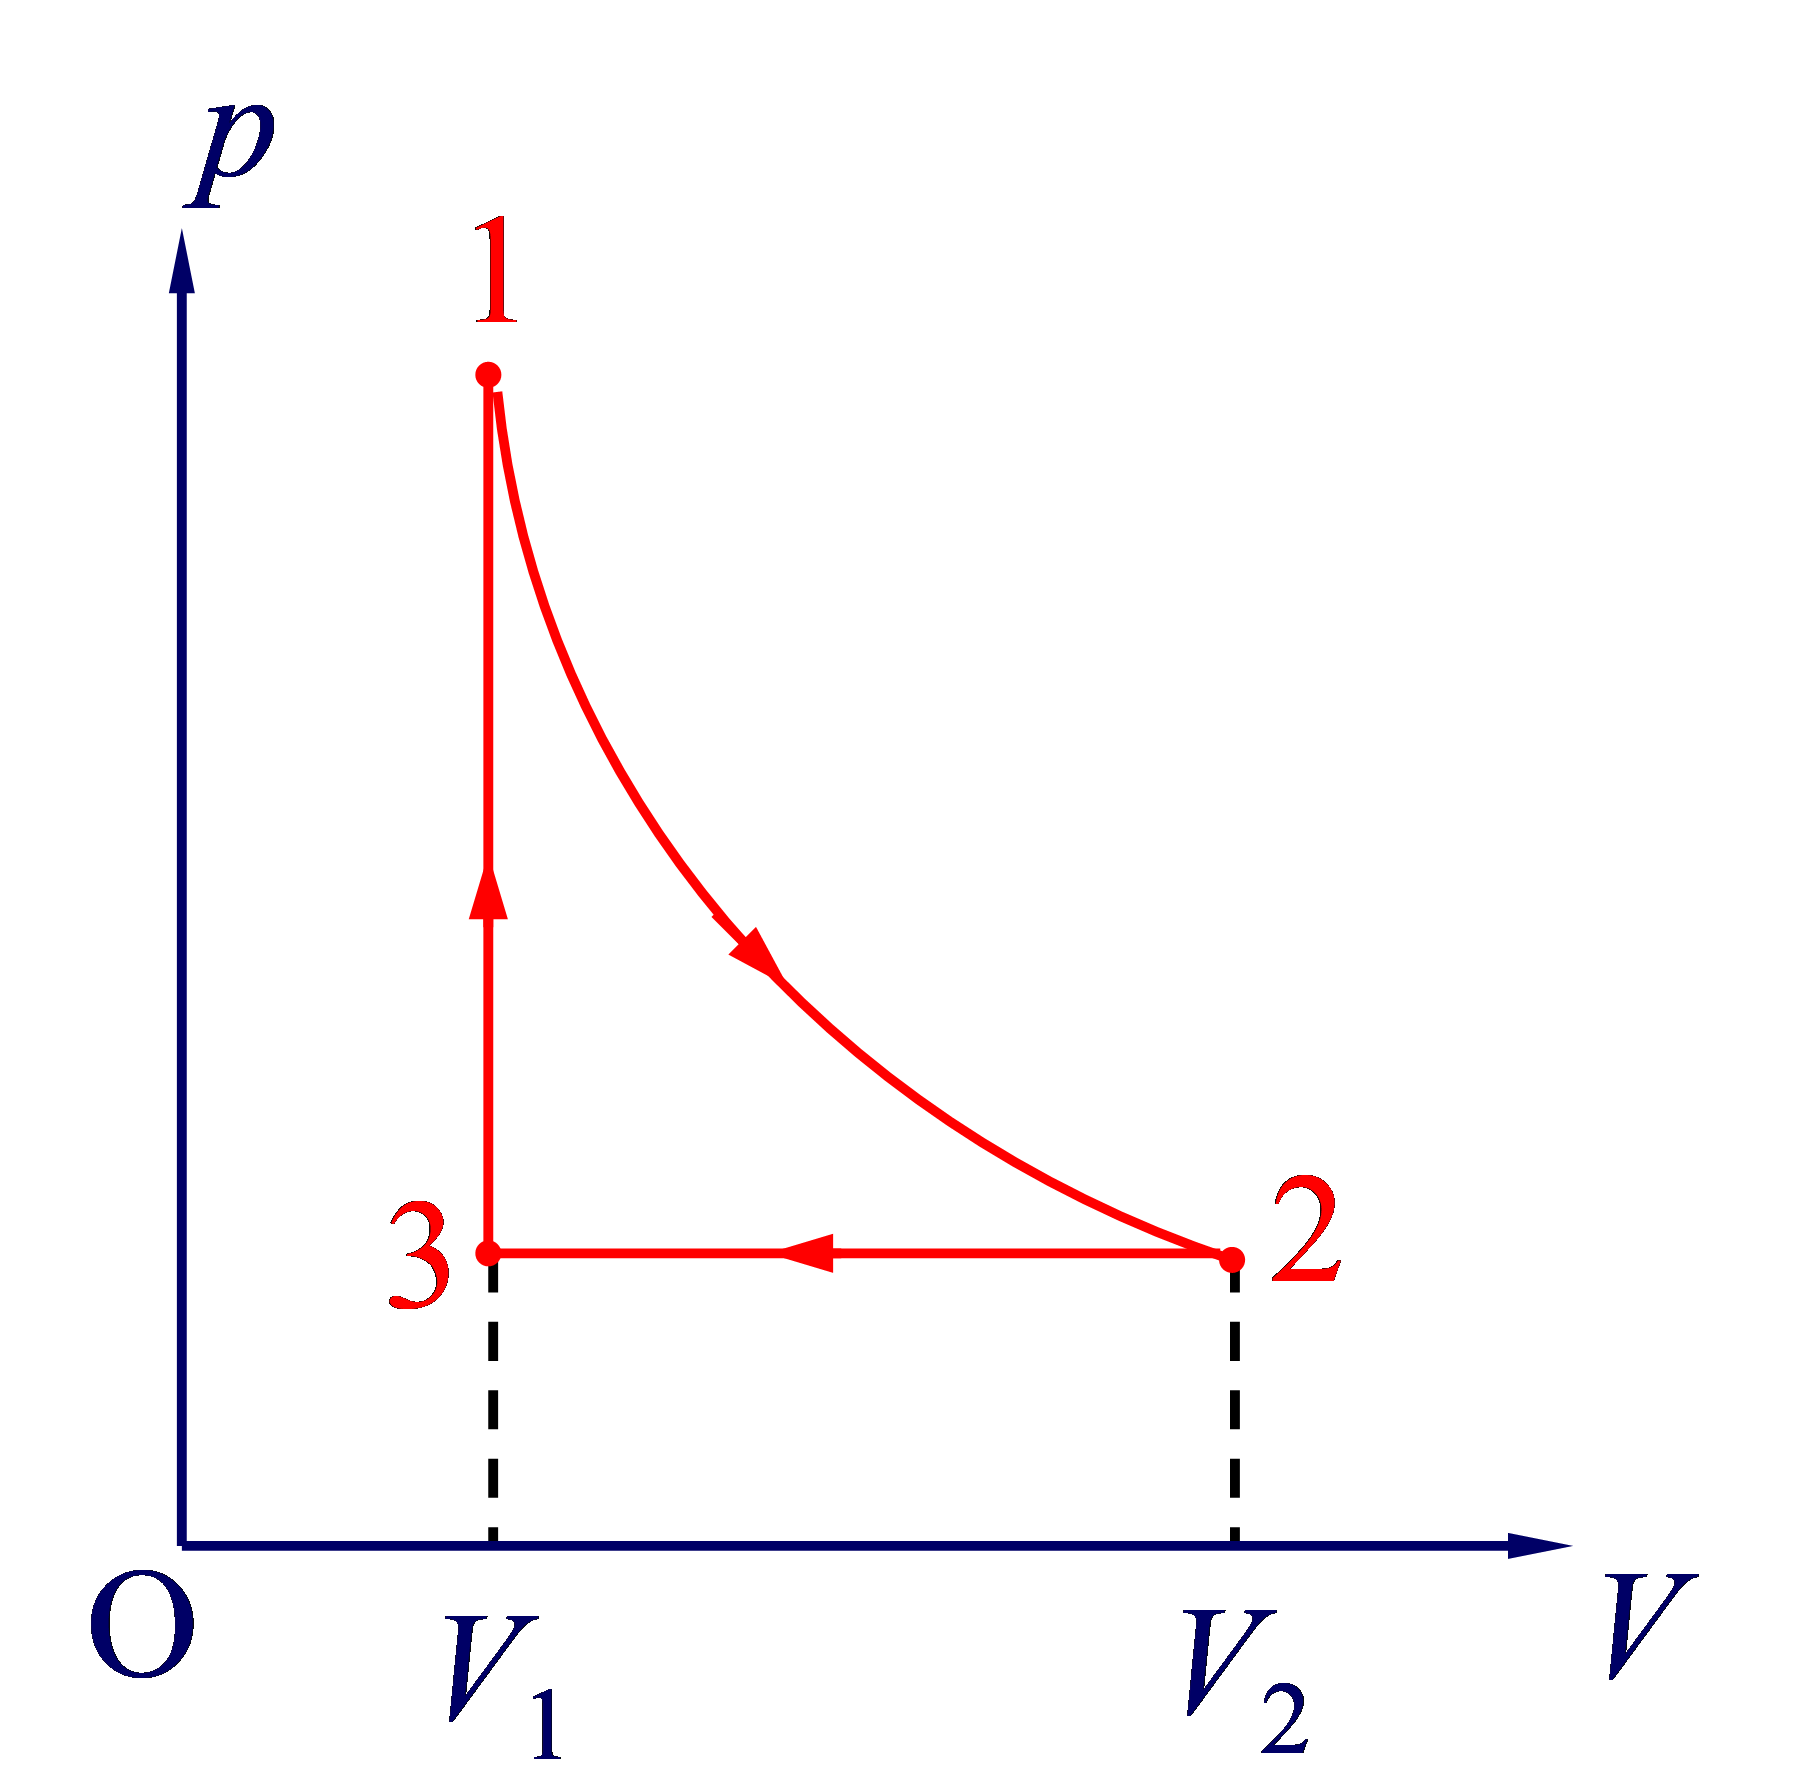
\includegraphics[width=5cm,height=4cm,keepaspectratio]{figures/image39.png}\par}\medskip

一热机的循环过程如图所示，其中 1\(\to\)2 为绝热过程，2\(\to\)3 为等压过程，3\(\to\)1 为等容过程。如工作物质为理想气体，其定容摩尔热容\(C_{V,m} = \frac{3}{2}R\)，\(V_{2} = 8V_{1}\)。

（1）求该热机的效率；

（2）若某一致冷机的循环过程为以上热机循环的逆循环，求该致冷机的致冷系数。

7．（10 分）

用一运转于\(T_{1} = 600K\)和\(T_{2} = 300K\)的高、低温热源之间的可逆热机推动一工作于\({T'}_{1} = 300K\)的热源和\({T'}_{2} = 250K\)的冷库之间的可逆冷机。为使制冷机每秒从冷库带走\(3.00 \times 10^{4}(J)\)的热量，热机每秒必须从高温热源吸收多少热量？

\end{document}
